\subsection{Adele 刻画}%
\label{sub:Adelic characterization}

回顾一下，在所有亏格中，GW不变量与GV不变量之间存在一个显式公式给出的关系。另一方面，我们可以通过 \(q \to 1\) 极限从KGW不变量恢复GW不变量。反方向则需要 Givental--Tonita的\textit{adelic characterization}~\cite{GiventalTonita2014}。其想法是，若有一个有理函数 \(f\)，则可以从它在单位根 \(\zeta\) 处的Laurent展开
\[ f_{q=\zeta} = \sum f_{\zeta, k} (1-\zeta^{-1} q)^k \]
将其恢复出来。

我们将研究惯性栈 \(I\bar{M}_{0,1}(X, \beta)\)。可以通过~\Cref{fig:givental-png}或~\Cref{fig:adelic-components}来记录其分支。
\begin{figure}[htpb]
    \centering
    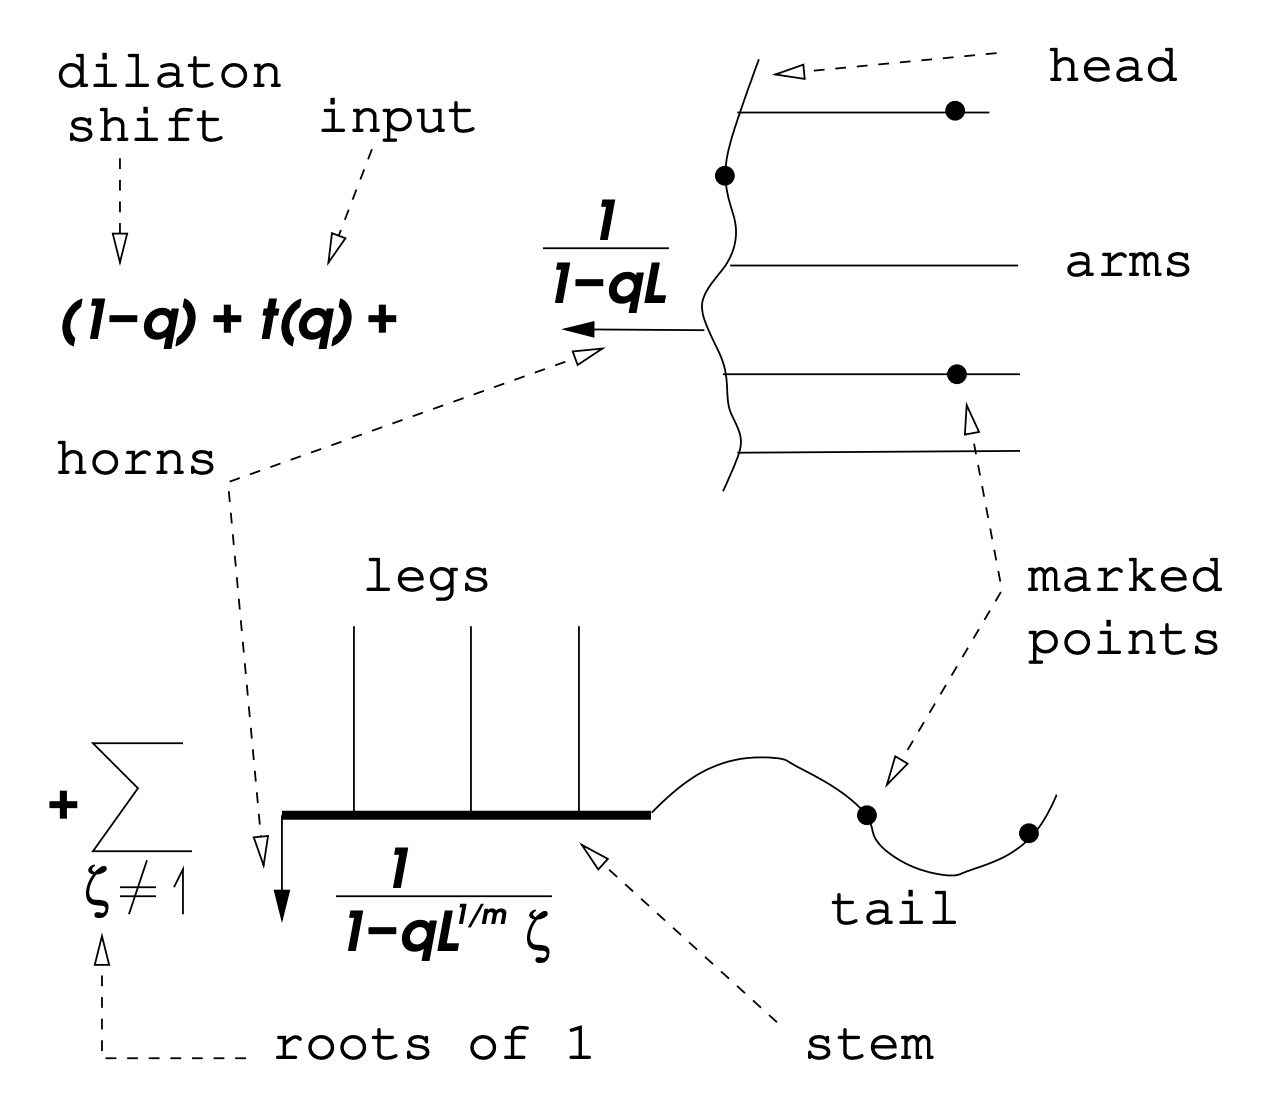
\includegraphics[width=0.8\textwidth]{givental.png}
    \caption{A way to keep track of the inertia components due to Givental-Tonita.}
    \label{fig:givental-png}
\end{figure}

\begin{figure}[htpb]
    \centering
    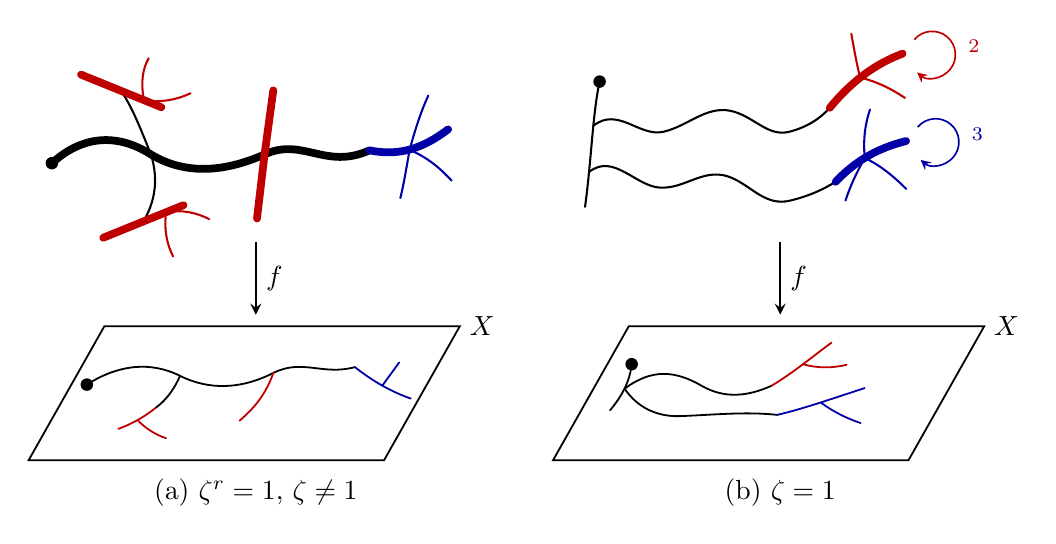
\begin{tikzpicture}[
        x=.74cm, y=.74cm,
        % Components of the domain curve. A cover style means the component
        % is a multiple cover of its image, drawn thick.
        dom/.style      ={black,         line width=.75pt, line cap=round},
        domcover/.style ={black,         line width=2.8pt, line cap=round},
        redcover/.style ={red!75!black,  line width=2.8pt, line cap=round},
        redtwig/.style  ={red!75!black,  line width=.75pt, line cap=round},
        bluecover/.style={blue!65!black, line width=2.8pt, line cap=round},
        bluetwig/.style ={blue!65!black, line width=.75pt, line cap=round},
        % Everything downstairs in X is drawn thin.
        img/.style      ={black,         line width=.65pt, line cap=round},
        redimg/.style   ={red!75!black,  line width=.65pt, line cap=round},
        blueimg/.style  ={blue!65!black, line width=.65pt, line cap=round},
        grparrow/.style ={->, >=stealth, line width=.6pt},
        fmap/.style     ={->, >=stealth, line width=.75pt},
        bull/.style     ={circle, fill=black, inner sep=1.6pt},
    ]

    %%%%%%%%%%%%%%%%%%%%%%%%%%%%%%%%%%%%%%%%%%%%%%%%%%%%%%%%%%%%%%%%%%%%%%%
    %% (a) zeta a primitive r-th root of unity, r >= 2.
    %%%%%%%%%%%%%%%%%%%%%%%%%%%%%%%%%%%%%%%%%%%%%%%%%%%%%%%%%%%%%%%%%%%%%%%
    \begin{scope}
        % The distinguished component: here g^r acts trivially on it, but g
        % does not, so it is a multiple cover of its image.
        \node[bull] at (-3.5,1.9) {};
        \draw[domcover]
            (-3.5,1.9)
            .. controls (-2.95,2.40) and (-2.35,2.40) .. (-1.80,2.05)
            .. controls (-1.25,1.72) and (-0.60,1.72) .. ( 0.15,2.05)
            .. controls ( 0.80,2.35) and ( 1.20,1.78) .. ( 1.95,2.12);

        % A leg meeting the distinguished component at a balanced node,
        % sticking out on both sides.  Each end carries a red multiple cover
        % together with the two branches interchanged by its automorphism.
        \draw[dom] (-1.80,2.05) .. controls (-2.00,2.55) and (-2.12,2.85) .. (-2.31,3.14);
        \draw[redcover] (-3.00,3.42) -- (-1.62,2.86);
        \draw[redtwig] (-1.92,2.98) .. controls (-1.98,3.30) and (-1.94,3.52) .. (-1.84,3.70);
        \draw[redtwig] (-1.92,2.98) .. controls (-1.62,2.94) and (-1.38,2.98) .. (-1.12,3.10);

        \draw[dom] (-1.80,2.05) .. controls (-1.66,1.60) and (-1.74,1.22) .. (-1.93,0.90);
        \draw[redcover] (-2.62,0.62) -- (-1.24,1.18);
        \draw[redtwig] (-1.54,1.06) .. controls (-1.58,0.74) and (-1.52,0.50) .. (-1.42,0.30);
        \draw[redtwig] (-1.54,1.06) .. controls (-1.26,1.10) and (-1.04,1.06) .. (-0.80,0.94);

        % A second balanced node, where the two legs are themselves the
        % multiple covers.
        \draw[redcover] (0.15,2.05) -- (0.30,3.15);
        \draw[redcover] (0.15,2.05) -- (0.02,0.95);

        % The tail: the part cut off at the unbalanced node.
        \draw[bluecover]
            (1.95,2.12) .. controls (2.45,2.02) and (2.85,2.14) .. (3.30,2.48);
        \draw[bluetwig] (2.64,2.13) .. controls (2.74,2.50) and (2.84,2.80) .. (2.96,3.06);
        \draw[bluetwig] (2.64,2.13) .. controls (2.58,1.80) and (2.54,1.54) .. (2.48,1.30);
        \draw[bluetwig] (2.64,2.13) .. controls (2.94,2.00) and (3.16,1.82) .. (3.36,1.60);

        \draw[fmap] (0,0.55) -- node[right] {$f$} (0,-0.70);

        % The target and the image of the map.
        \draw[img] (-3.9,-3.2) -- (2.2,-3.2) -- (3.5,-0.9) -- (-2.6,-0.9) -- cycle;
        \node[right] at (3.5,-0.9) {$X$};
        \node[bull] at (-2.90,-1.90) {};
        \draw[img] (-2.90,-1.90)
            .. controls (-2.35,-1.55) and (-1.80,-1.50) .. (-1.30,-1.75)
            .. controls (-0.80,-2.00) and (-0.25,-1.98) .. ( 0.30,-1.70)
            .. controls ( 0.80,-1.45) and ( 1.15,-1.75) .. ( 1.70,-1.60);
        % The two branches upstairs are folded onto the single one downstairs.
        \draw[img]    (-1.30,-1.75) .. controls (-1.42,-2.02) and (-1.56,-2.18) .. (-1.72,-2.30);
        \draw[redimg] (-1.72,-2.30) .. controls (-1.92,-2.46) and (-2.14,-2.58) .. (-2.36,-2.66);
        \draw[redimg] (-2.02,-2.52) .. controls (-1.88,-2.66) and (-1.72,-2.76) .. (-1.54,-2.82);
        \draw[redimg] ( 0.30,-1.70) .. controls ( 0.18,-2.05) and (-0.02,-2.30) .. (-0.28,-2.52);
        \draw[blueimg] (1.70,-1.60) .. controls (2.02,-1.85) and (2.32,-2.02) .. (2.66,-2.14);
        \draw[blueimg] (2.17,-1.92) .. controls (2.27,-1.78) and (2.36,-1.66) .. (2.46,-1.52);

        \node at (0,-3.75) {(a) \(\zeta^r = 1\), \(\zeta \neq 1\)};
    \end{scope}

    %%%%%%%%%%%%%%%%%%%%%%%%%%%%%%%%%%%%%%%%%%%%%%%%%%%%%%%%%%%%%%%%%%%%%%%
    %% (b) zeta = 1.
    %%%%%%%%%%%%%%%%%%%%%%%%%%%%%%%%%%%%%%%%%%%%%%%%%%%%%%%%%%%%%%%%%%%%%%%
    \begin{scope}[shift={(9,0)}]
        % Now g acts trivially on the distinguished component, so it is drawn
        % thin: it maps isomorphically onto its image.
        \node[bull] at (-3.10,3.30) {};
        \draw[dom] (-3.10,3.30) .. controls (-3.22,2.75) and (-3.24,1.95) .. (-3.35,1.15);
        \draw[dom] (-3.21,2.54)
            .. controls (-2.78,2.88) and (-2.42,2.34) .. (-2.00,2.44)
            .. controls (-1.58,2.54) and (-1.28,2.88) .. (-0.86,2.80)
            .. controls (-0.46,2.72) and (-0.22,2.34) .. ( 0.16,2.44)
            .. controls ( 0.46,2.52) and ( 0.68,2.66) .. ( 0.85,2.85);
        \draw[dom] (-3.28,1.75)
            .. controls (-2.86,2.08) and (-2.48,1.50) .. (-2.06,1.48)
            .. controls (-1.64,1.46) and (-1.34,1.80) .. (-0.92,1.68)
            .. controls (-0.52,1.56) and (-0.28,1.14) .. ( 0.18,1.26)
            .. controls ( 0.50,1.34) and ( 0.72,1.44) .. ( 0.95,1.58);

        % The arms: g acts nontrivially on them, through the indicated cyclic
        % group, which interchanges the thin branches sticking out.
        \draw[redcover] (0.85,2.85) .. controls (1.22,3.30) and (1.62,3.60) .. (2.10,3.78);
        \draw[redtwig] (1.37,3.37) .. controls (1.30,3.66) and (1.26,3.90) .. (1.22,4.12);
        \draw[redtwig] (1.37,3.37) .. controls (1.66,3.30) and (1.90,3.18) .. (2.14,3.02);
        \draw[grparrow, red!75!black]
            (2.30,4.02) arc[start angle=140, end angle=-130, radius=.40];
        \node[red!75!black, right] at (3.06,3.90) {$\Z_2$};

        \draw[bluecover] (0.95,1.58) .. controls (1.30,1.95) and (1.68,2.16) .. (2.16,2.28);
        \draw[bluetwig] (1.45,1.99) .. controls (1.42,2.32) and (1.46,2.58) .. (1.54,2.82);
        \draw[bluetwig] (1.45,1.99) .. controls (1.72,1.86) and (1.94,1.68) .. (2.16,1.46);
        \draw[bluetwig] (1.45,1.99) .. controls (1.30,1.72) and (1.20,1.50) .. (1.12,1.26);
        \draw[grparrow, blue!65!black]
            (2.36,2.52) arc[start angle=140, end angle=-130, radius=.40];
        \node[blue!65!black, right] at (3.12,2.40) {$\Z_3$};

        \draw[fmap] (0,0.55) -- node[right] {$f$} (0,-0.70);

        % The target and the image of the map.
        \draw[img] (-3.9,-3.2) -- (2.2,-3.2) -- (3.5,-0.9) -- (-2.6,-0.9) -- cycle;
        \node[right] at (3.5,-0.9) {$X$};
        \node[bull] at (-2.55,-1.55) {};
        \draw[img] (-2.55,-1.55) .. controls (-2.58,-1.85) and (-2.72,-2.10) .. (-2.92,-2.34);
        \draw[img] (-2.67,-1.97)
            .. controls (-2.20,-1.62) and (-1.80,-1.66) .. (-1.35,-1.92)
            .. controls (-0.95,-2.15) and (-0.55,-2.10) .. (-0.15,-1.92);
        \draw[img] (-2.67,-1.97)
            .. controls (-2.45,-2.30) and (-2.10,-2.46) .. (-1.70,-2.44)
            .. controls (-1.15,-2.42) and (-0.60,-2.36) .. (-0.05,-2.42);
        % Each arm is folded onto a single image curve with one branch.
        \draw[redimg] (-0.15,-1.92) .. controls (0.25,-1.68) and (0.55,-1.42) .. (0.88,-1.18);
        \draw[redimg] ( 0.39,-1.55) .. controls (0.63,-1.62) and (0.89,-1.62) .. (1.14,-1.56);
        \draw[blueimg] (-0.05,-2.42) .. controls (0.45,-2.30) and (0.95,-2.12) .. (1.45,-1.96);
        \draw[blueimg] ( 0.70,-2.21) .. controls (0.90,-2.36) and (1.14,-2.48) .. (1.38,-2.56);

        \node at (0,-3.75) {(b) \(\zeta = 1\)};
    \end{scope}
    \end{tikzpicture}
    \caption{\(I\bar{M}_{0,1}(X,\beta)\) 的分支，归功于You-Cheng。}
    \label{fig:adelic-components}
\end{figure}

下面我们解释~\Cref{fig:adelic-components}。设 \(L_1\) 为第一个标记点处的余切线，设 \(g\) 为 \(I\bar{M}_{0,1}(X,\beta)\) 中一点的自同构。则 \(\zeta\) 由 \(g\) 在 \(L_1\) 上以特征值 \(\zeta\) 作用这一条件定义。在两幅图中，圆点表示第一个标记点及其在 \(X\) 中的像，而粗分支表示它是其像的多重覆盖。

首先，假设 \(\zeta = 1\)。此时黑色分支是包含第一个标记点的极大连通分支，\(g\) 在其上作用为恒等。红色和蓝色分支正是 \(g\) 非平凡作用的分支，我们称之为\textit{臂}。

现在假设 \(\zeta\) 是某个 \(r \geq 2\) 的 \(r\) 次单位根。此时要求黑色分支的节点关于 \(g\) 作用是平衡的，因此我们切掉非平衡部分，即图中蓝色部分，并称之为\textit{尾}。在剩余部分中，黑色分支是包含第一个标记点的极大连通分支，\(g^r\) 在其上作用为恒等。最后，在去掉黑色分支和尾之后，剩下的分支称为\textit{腿}。

% \begin{figure}[htpb]
%     \centering
%     \resizebox{\textwidth}{!}{%
%     \begin{tikzpicture}[
%         x=1cm,
%         y=1cm,
%         curve/.style={black, line width=1.25pt, line cap=round},
%         fixed component/.style={black, line width=3.2pt, line cap=round},
%         red component/.style={red!75!black, line width=3.2pt, line cap=round},
%         blue component/.style={blue!70!black, line width=3.2pt, line cap=round},
%         image curve/.style={black, line width=1.05pt, line cap=round},
%         action arrow/.style={->, >=stealth, line width=.75pt},
%         map arrow/.style={->, >=stealth, line width=.8pt},
%         marked point/.style={circle, fill=black, inner sep=1.8pt}
%     ]
%         % The case of a nontrivial r-th root of unity.
%         \begin{scope}[xshift=0cm]
%             \node[font=\large] at (0,5.95)
%                 {$r\geq 2,\qquad \zeta^r=1,\quad \zeta\neq 1$};
%
%             % Domain curve.
%             \node[marked point] (p1) at (-3.15,3.7) {};
%             \draw[fixed component]
%                 (p1) .. controls (-2.25,4.15) and (-1.55,4.2) ..
%                 (-1.15,3.92)
%                 .. controls (-0.55,3.45) and (0.35,3.45) ..
%                 (0.85,3.82)
%                 .. controls (1.35,3.35) and (1.85,3.45) ..
%                 (2.2,4.05);
%             \fill (-1.15,3.92) circle (2.2pt);
%             \fill (0.85,3.82) circle (2.2pt);
%             \fill (2.2,4.05) circle (2.2pt);
%
%             % Two legs attached to balanced nodes.
%             \draw[curve]
%                 (-1.15,3.92) .. controls (-1.25,4.45) and (-1.35,4.78) ..
%                 (-1.72,5.18);
%             \draw[red component]
%                 (-2.18,5.48) .. controls (-1.92,5.25) and (-1.65,5.08) ..
%                 (-1.36,5.02);
%             \draw[curve, red!75!black]
%                 (-1.67,5.14) .. controls (-1.64,5.35) and (-1.59,5.55) ..
%                 (-1.53,5.72);
%             \draw[curve, red!75!black]
%                 (-1.53,5.08) .. controls (-1.34,5.14) and (-1.18,5.25) ..
%                 (-1.02,5.4);
%             \draw[action arrow, red!75!black]
%                 (-1.9,5.38) arc[start angle=20,end angle=315,radius=.42];
%
%             \draw[curve]
%                 (-1.15,3.92) .. controls (-1.1,3.35) and (-1.25,3.0) ..
%                 (-1.62,2.63);
%             \draw[red component]
%                 (-2.18,2.32) .. controls (-1.9,2.56) and (-1.6,2.75) ..
%                 (-1.3,2.84);
%             \draw[curve, red!75!black]
%                 (-1.65,2.68) .. controls (-1.62,2.48) and (-1.59,2.25) ..
%                 (-1.54,2.06);
%             \draw[curve, red!75!black]
%                 (-1.5,2.76) .. controls (-1.31,2.7) and (-1.14,2.58) ..
%                 (-.98,2.42);
%             \draw[action arrow, red!75!black]
%                 (-1.85,2.57) arc[start angle=25,end angle=315,radius=.38];
%
%             % A second symmetric pair of balanced legs.
%             \draw[curve] (0.2,3.48) .. controls (0.16,4.05) and (0.2,4.35) ..
%                 (0.32,4.7);
%             \draw[red component] (0.2,3.9) -- (0.33,4.72);
%             \draw[curve] (0.2,3.48) .. controls (0.16,3.12) and (0.08,2.82) ..
%                 (-0.02,2.48);
%             \draw[red component] (0.11,3.05) -- (-0.03,2.46);
%
%             % The nonbalanced tail.
%             \draw[blue component]
%                 (2.2,4.05) .. controls (2.68,3.92) and (3.05,4.02) ..
%                 (3.48,4.3);
%             \draw[curve, blue!70!black] (2.86,4.08) -- (3.15,4.78);
%             \draw[curve, blue!70!black] (2.95,4.07) -- (2.88,3.35);
%             \draw[curve, blue!70!black] (2.95,4.07) -- (3.45,3.55);
%
%             % The target and the image of the map.
%             \draw[curve]
%                 (-3.55,-1.65) -- (2.48,-1.65) -- (3.48,1.0) --
%                 (-2.65,1.0) -- cycle;
%             \node[marked point] (xp1) at (-2.65,-0.25) {};
%             \draw[image curve]
%                 (xp1) .. controls (-2.05,0.04) and (-1.55,.22) ..
%                 (-1.15,.12)
%                 .. controls (-.5,-.05) and (-.2,-.1) ..
%                 (.12,.18)
%                 .. controls (.55,.55) and (1.0,.62) ..
%                 (1.55,.45);
%             % The first red orbit maps to a black connector followed by
%             % one red image curve; its two thin branches fold to the
%             % smaller red branch.
%             \draw[image curve]
%                 (-1.15,.12) .. controls (-1.23,-.08) and (-1.34,-.23) ..
%                 (-1.48,-.32);
%             \draw[red!75!black, line width=1.05pt, line cap=round]
%                 (-1.48,-.32) .. controls (-1.62,-.45) and (-1.78,-.58) ..
%                 (-1.92,-.65);
%             \draw[red!75!black, line width=1.05pt, line cap=round]
%                 (-1.69,-.51) .. controls (-1.58,-.64) and (-1.45,-.72) ..
%                 (-1.31,-.76);
%             \draw[red!75!black, line width=1.05pt, line cap=round]
%                 (.12,.18) .. controls (.02,-.22) and (-.25,-.38) ..
%                 (-.48,-.63);
%             \draw[blue!70!black, line width=1.05pt, line cap=round]
%                 (1.05,.57) .. controls (1.35,.12) and (1.68,-.18) ..
%                 (2.08,-.38);
%             \draw[blue!70!black, line width=1.05pt, line cap=round]
%                 (1.78,-.2) .. controls (1.82,-.08) and (1.88,.04) ..
%                 (1.96,.15);
%             \draw[map arrow] (0,2.62) -- node[right] {$f$} (0,1.22);
%             \node at (0,-2.1) {$(a)\ \zeta\neq 1$};
%         \end{scope}
%
%         % The untwisted eigenvalue case.
%         \begin{scope}[xshift=8.25cm]
%             \node[font=\large] at (0,5.95)
%                 {$I\overline{\mathcal M}_{0,1}(X,\beta),\qquad
%                   \on{Tr} g|_{L_1}=\zeta$};
%
%             % Domain curve: the thick portions have multiple covers onto
%             % their images.
%             \node[marked point] (p2) at (-2.95,4.45) {};
%             \draw[fixed component]
%                 (p2) .. controls (-3.08,3.85) and (-3.08,3.18) ..
%                 (-3.18,2.65);
%             \draw[curve]
%                 (-3.02,3.9) .. controls (-2.42,4.05) and (-2.0,3.62) ..
%                 (-1.62,3.72)
%                 .. controls (-1.18,3.3) and (-.72,3.18) ..
%                 (-.2,3.32);
%             \draw[curve]
%                 (-3.13,3.25) .. controls (-2.6,3.52) and (-2.25,2.88) ..
%                 (-1.8,2.68)
%                 .. controls (-1.25,2.4) and (-.68,2.42) ..
%                 (-.15,2.48);
%
%             % Nontrivial arms, shown in red and blue.
%             \draw[curve]
%                 (-.2,3.32) .. controls (.3,3.48) and (.5,3.72) ..
%                 (.76,3.92);
%             \draw[red component]
%                 (.76,3.92) .. controls (1.1,4.42) and (1.5,4.72) ..
%                 (2.02,4.9);
%             \draw[curve, red!75!black]
%                 (1.12,4.4) .. controls (1.08,4.68) and (1.05,4.92) ..
%                 (1.02,5.18);
%             \draw[curve, red!75!black]
%                 (1.55,4.7) .. controls (1.82,4.62) and (2.04,4.48) ..
%                 (2.25,4.3);
%             \draw[action arrow, red!75!black]
%                 (1.6,4.88) arc[start angle=210,end angle=-35,radius=.48];
%             \node[red!75!black, left] at (1.02,5.08) {$\Z_2$};
%
%             \draw[curve]
%                 (-.15,2.48) .. controls (.28,2.45) and (.55,2.64) ..
%                 (.86,2.76);
%             \draw[blue component]
%                 (.86,2.76) .. controls (1.18,3.13) and (1.52,3.32) ..
%                 (2.0,3.42);
%             \draw[curve, blue!70!black]
%                 (1.27,3.13) .. controls (1.34,3.4) and (1.43,3.65) ..
%                 (1.55,3.9);
%             \draw[curve, blue!70!black]
%                 (1.57,3.33) .. controls (1.83,3.2) and (2.05,3.02) ..
%                 (2.27,2.82);
%             \draw[action arrow, blue!70!black]
%                 (1.9,3.37) arc[start angle=145,end angle=-120,radius=.43];
%             \node[blue!70!black, above] at (2.55,3.62) {$\Z_3$};
%
%             % Target X and the images of the colored components.
%             \draw[curve]
%                 (-3.55,-1.65) -- (2.48,-1.65) -- (3.48,1.0) --
%                 (-2.65,1.0) -- cycle;
%             \node[marked point] (xp2) at (-2.05,.02) {};
%             \draw[image curve]
%                 (xp2) .. controls (-2.0,-.32) and (-2.35,-.62) ..
%                 (-2.62,-.93);
%             \draw[image curve]
%                 (-2.25,-.52) .. controls (-1.82,-.12) and (-1.55,-.12) ..
%                 (-1.14,-.42)
%                 .. controls (-.88,-.62) and (-.54,-.63) ..
%                 (-.22,-.52);
%             \draw[image curve]
%                 (-2.25,-.52) .. controls (-2.58,-.44) and (-2.75,-.62) ..
%                 (-2.98,-.83);
%             \draw[red!75!black, line width=1.05pt]
%                 (-.22,-.52) .. controls (.22,-.13) and (.5,.22) ..
%                 (.82,.48);
%             % The two thin red branches upstairs fold to this one
%             % additional branch of the red image curve.
%             \draw[red!75!black, line width=1.05pt, line cap=round]
%                 (.345,.029) .. controls (.57,-.02) and (.77,.06) ..
%                 (1.0,.18);
%             % A chain of black components joins the blue image to the
%             % distinguished black component.
%             \draw[image curve]
%                 (-2.25,-.52) .. controls (-2.12,-.76) and (-2.0,-.91) ..
%                 (-1.88,-1.0);
%             \draw[image curve]
%                 (-1.88,-1.0) .. controls (-1.76,-.82) and (-1.53,-.91) ..
%                 (-1.38,-1.18);
%             \draw[image curve]
%                 (-1.38,-1.18) .. controls (-.65,-.76) and (.08,-.68) ..
%                 (.78,-.72);
%             \draw[blue!70!black, line width=1.05pt, line cap=round]
%                 (.78,-.72) .. controls (1.24,-.74) and (1.58,-.62) ..
%                 (1.98,-.32);
%             \draw[map arrow] (0,2.03) -- node[right] {$f$} (0,1.22);
%             \node at (0,-2.1) {$(b)\ \zeta=1$};
%         \end{scope}
%     \end{tikzpicture}%
%     }
%     \caption{The decomposition of a component of
%     \(I\overline{\mathcal M}_{0,1}(X,\beta)\) into its distinguished
%     component, legs or arms, and tail, provided by You-Cheng. Thick curves indicate components
%     that map with degree greater than one onto their images. Symmetric
%     branches occur on the domain, and \(f\) folds each orbit to a single
%     image curve in \(X\).}
%     \label{fig:adelic-components}
% \end{figure}
%
% We will now explain the meaning of the different parts of~\Cref{fig:adelic-components}. Let \(L_1\)
% be the cotangent line at the first marked point and define \(\zeta\) by
% \[
%     g|_{L_1}=\zeta\,\mr{Id}_{L_1}.
% \]
% The bullets denote the first marked point and its image in \(X\), and a
% thick curve denotes a component that is a multiple cover of its image.
% The black component is the maximal connected component containing the
% first marked point on which \(g\) acts trivially when \(\zeta=1\). The red
% and blue components on which \(g\) acts nontrivially are called
% \textit{arms}.
%
% More generally, suppose that \(\zeta\) is an \(r\)-th root of unity with
% \(r\geq 2\). The nodes of the thick black component must be balanced with
% respect to the \(g\)-action. Cut off the part attached at an unbalanced
% node (the blue component in the figure); this part is called the
% \textit{tail}. In what remains, the thick black component is the maximal
% connected component containing the first marked point on which \(g^r\)
% acts trivially. After removing the black component and the tail, the
% remaining components are called \textit{legs}.

下面的定义归功于Givental。我们记
\[ \ab<\frac{\Phi}{1-qL}>_{0,1,\beta}^{X,K} \coloneqq \sum_{\zeta} \ab<\frac{\Phi}{1-qL}>_{0,1,\beta}^{X_{\zeta}}, \]
其中 \(X_{\zeta}\) 项即为 \(M_{\zeta}\) 在Riemann-Roch定理下的贡献。现在，我们来定义臂、腿和尾。在此，我们定义\textit{臂}
\[ \mr{arm}(q) \coloneqq \sum_{\beta, \alpha, \zeta \neq 1} Q^{\beta} \Phi^{\alpha}\ab<\frac{\Phi_{\alpha}}{1-qL}>_{0,1,\beta}^{X_{\zeta}}, \]
\textit{腿}
\[ \mr{leg}_{\zeta}(q) \coloneqq \mr{leg}_r(q) = \Psi^r (\mr{arm}(q)), \]
以及\textit{尾}
\[ \mr{tail}_{\zeta}(q) \coloneqq \sum_{\beta, \alpha, \zeta' \neq \zeta} Q^{\beta} \Phi^{\alpha} \ab<\frac{\Phi_{\alpha}}{1-qL}>_{0,1,\beta}^{X_{\zeta'}}. \]

\begin{prop}[{\cite{GiventalTonita2014}}]
    J函数在 \(q = 1\) 处的Laurent展开由下式给出
    \begin{align*}
        J^K(0)_{q=1} &= J^{\mr{fake}}(\mr{arm}(q)) \\
        &\coloneqq 1-q + \mr{arm}(q) + \sum_{n,\beta,\alpha} \frac{Q^{\beta}\Phi^{\alpha}}{n!} \ab<\frac{\Phi_{\alpha}}{1-qL}, \mr{arm}(L), \ldots, \mr{arm}(L)>_{0,n+1,\beta}^{\mr{fake}},
    \end{align*}
    其中fake不变量通过应用Riemann-Roch并仅考虑非扭分支的贡献来计算。
\end{prop}

\begin{prop}[{\cite{GiventalTonita2014}}]
    在任一其它单位根 \(\zeta \neq 1\) 处，我们有
    \begin{align*}
        &J^K(0)_{q = \zeta} = (1-q) + \mr{tail}_{\zeta}(q) \\
        &+ \sum_{n,\beta,\alpha} \frac{Q^{r\beta}\Phi^{\alpha}}{n!} \ab[\frac{\Phi_{\alpha}}{1-\zeta q L^{1/r}}, \mr{leg}_r(L), \ldots, \mr{leg}_r(L), 1 - \zeta^{-1}L^{1/r} + \mr{tail}_{\zeta}(\zeta^{-1} L^{1/r})]^{\mr{stem}},
    \end{align*}
    其中stem是定义在模空间上的 \(X \times B\mu_r\) 的某种fake不变量
    \[ \bar{M}_{0,n+2,\beta}^X(\zeta) \coloneqq \bar{M}_{0,n+2}(X \times B\mu_r, \beta, (g, 1, \ldots, 1, g^{-1})). \]
    它由如下公式定义
    \begin{align*}
        [\cdots]^{\mr{stem}} \coloneqq \int_{[\bar{M}_{0,n+2,\beta}^X(\zeta)]^{\vir}} \on{td}(T_{\bar{M}}) \on{ch}\ab(\frac{\on{Tr}(\cdots)}{\on{Tr}(\lambda_{-1}(N^*))}),
    \end{align*}
    其中 \(N\) 表示 \(\bar{M}_{0,n+2,\beta}^X(\zeta) \subset \bar{M}_{0,nr+2}(X, r\beta)\) 的法丛。
\end{prop}

\begin{rmk}
    如果我们能计算fake理论和stem理论，那么就能计算亏格零的量子K不变量。
\end{rmk}

\subsection{点的量子 K-理论}%
\label{sub:Quantum K-theory of a point}

一个自然的问题是研究高亏格量子K理论。我们将从最简单的目标，即一个点开始。研究高亏格的一个动机是试图证明Calabi-Yau四流形的Klemm-Pandharipande定义的GV不变量，或Calabi-Yau五流形的Pandharipande-Zinger定义的GV不变量的整性（在这种情形下，我们只需考虑亏格 \(1\)）。我们需要考虑点的量子K理论的一个原因是，在 \(I\bar{M}_{1,1}(X, \beta)\) 中，存在一些分支，其中整条亏格 \(1\) 曲线被收缩为一个点。

\begin{quest}
    K理论的Witten-Kontsevich定理是什么？\footnote{According to You-Cheng, the difficulty lies everywhere.}
\end{quest}

我们先回顾上同调的Witten猜想。我们先从算子
\[ L = \partial_x^2 + u(x) \]
出发，将其形变为
\[ \tilde{L} = \partial_x^2 + u(x, T_3, T_5, \ldots), \]
其中应把 \(x = T_1\) 且 \(u(x) = u(x, 0, 0,\ldots)\) 理解为初始条件。形式地写
\[ L^{1/2} = \partial_x + \sum_{k > 0} a_{-k}(x) \partial_x^{-k} \]
利用性质
\[ \partial^n \circ f = \sum_{m = 0}^{\infty} \binom{n}{m} f^{(m)} \partial^{n-m} \]
对一切整数 \(n \in \Z\) 成立。特别地，我们由方程构造(2-)KdV层级
\[ \pdv{\tilde{L}}{T_{2k+1}} = \ab[(\tilde{L}^{\frac{2k+1}{2}})_{\geq 0}, \tilde{L}] \]
对一切 \(k \geq 0\) 成立。我们称函数 \(\tau\) 为\textit{\(\tau\)-函数}，若
\[ 2 \pdv[2]{}{x}\log \tau(x, T_3, T_5, \ldots) = u(x, T_3, T_5, \ldots). \]
现在用 \(u = 2x\) 进行上述过程。定义函数
\[ F(t_0, t_1, \ldots) \coloneqq \sum_{n \geq 0} \sum_{k_0, \ldots, k_n} \ab<\tau_0^{k_0} \cdots \tau_n^{k_n}> \frac{t_0^{k_0} \cdots t_n^{k_n}}{k_0! \cdots k_n!}. \]
注意，由于亏格完全由插入点的个数和插入点的次数决定，记号
\[ \ab<\tau_0^{k_0} \cdots \tau_n^{k_n}> \]
唯一确定了一个点的后代GW不变量。

\begin{thm}[Kontsevich {\cite{Kontsevich1992}}]
    在变量替换 \(t_i = (2i+1)!! T_{2i+1}\) 下，\(F\) 是从 \(L = \partial_x^2 + 2x\) 出发构造的KdV层级的一个 \(\tau\)-函数。
\end{thm}

该定理的一个应用是考虑虚拟局部化。例如，假设考虑 \(\bar{M}_{g,0}(X, d[C])\)，其中 \(C\) 是Calabi-Yau三流形中法丛为 \(N = \mc{O}(-1)\oplus \mc{O}(-1)\) 的唯一有理曲线。此时在此设定下我们可以约化到局部模型并计算
\begin{align*}
    \int_{[\bar{M}_{g,0}(\P^1, d)]^{\vir}} c_{\mr{top}}(R^1 \pi_* N) = \sum_{m \vdash d} \frac{(-1)^{d-L(m)}}{\abs{\Aut(m)}} \int_{\bar{M}_{g, L(m)}} \frac{1 + \cdots + c_g(\mc{H})}{\prod_i (1-m_i \psi_i)}
\end{align*}
通过虚拟局部化。若希望在K理论中有类似结果，则需考虑形如
\[ \chi\ab(\bar{M}_{g, L(m)}/\Aut(m), \frac{\lambda_{-1}(\mc{H})}{1-m_i L_i}), \]
的项，因此需要考虑点的置换等变量子K理论。

我们现在进行文献综述。首先，Lee~\cite{Lee1997}计算了公式
\[ \ab<\frac{1}{1-q_1 L}, \ldots, \frac{1}{1-q_n L}>_{0,n}^{\mr{pt}, K} = \ab(\prod_{i=1}^n \frac{1}{1-q_i}) \ab(1 + \sum_{i=1}^n \frac{q_i}{1-q_i})^{n-3}. \]
后来，Lee--Qu~\cite{LeeQu2014}原则上给出了计算
\[ \ab<\frac{1}{1-q_1 L}, \ldots, \frac{1}{1-q_n L}>_{1,n}^{\mr{pt}, K} \]
的方法。Givental~\cite{Givental2017K1}计算了公式
\[ \sum_{n \geq 2} \ab<\frac{1}{1-q L}, 1, \ldots, 1>_{0,1+n}^{S_n} = (1-q) \exp\ab(\sum_{k > 0} \frac{\Psi^k}{k} \ab(1 + \frac{q}{1-q})). \]
最后，Milanov~\cite{Milanov2025}在一篇2024年首次发布的预印本中计算了
\begin{align*}
    \sum_{n \geq 0}& \ab<\frac{1}{1-q_1 L}, \ldots, \frac{1}{1-q_r L}, 1, \ldots, 1>_{0,r+n}^{S_n} \\
    &= \ab(\prod_{i=1}^{r} \frac{1}{1-q_i})\ab(1 + \sum_{i=1}^r \frac{q_i}{1-q_i}) \exp\ab(\sum_{k > 0} \frac{\Psi^k}{k} \ab(1 + \sum_{i=1}^r \frac{q_i}{1-q_i})).
\end{align*}

下面的多重Hodge递推以及基于它们的新亏格一计算归功于周宥承，并在本次讲座中报告。

设 \(s \in \Z\) 并定义多重Hodge层 \(\mc{H}_s \coloneqq R^0 \pi_* (\omega_{\pi}^s)\)。考虑映射 \(\bar{M}_{g,n+1} \xrightarrow{\pi} \bar{M}_{g,n}\)，我们将上层的余切线记为 \(L_i\)，下层的记为 \(\ell_i\)。

\begin{lem}
    对一切整数 \(s\) 和 \(d_i\)，我们有
    \[ \pi_*\ab(\omega_{\pi}^s\ab(\sum_{i=1}^n d_i D_i)) = \mc{H}_s-\mc{H}_{1-s}^* + \sum_{i=1}^n \sum_{k=1}^{d_i} \ell_i^{-k+s}. \]
\end{lem}

\begin{rmk}
    注意，若 \(f(q) \in \Z[q]\)，则 \(\exp \sum_k \frac{\Psi^k}{k} (f(q)) \in \Z \ps{q}\)。原因是该运算把 \(f = \sum_{i=1}^{n} a_i q^i\) 映为 \(\prod_{i=1}^n \frac{1}{(1-q^i)^{a_i}}\)。
\end{rmk}

\begin{proof}
    当所有 \(d_i\) 均为零时，我们看到
    \[ R^0 \pi_* \omega_{\pi}^s - R^1 \pi_* \omega_{\pi}^s = \mc{H}_s - \mc{H}_{1-s}^* \]
    由Serre对偶得到。下一步是证明
    \[ \pi_* \omega_{\pi}^s ((r+1)D_i) = \pi_* \omega_{\pi}^s(r D_i) + \ell_i^{s-r-1}. \]
    在此，我们先考虑正合列
    \[ 0 \to \mc{O} (-D_i) \to \mc{O} \to \mc{O}_{D_i} \to 0 \]
    并用 \(\omega_{\pi}^s\) 扭转得到
    \[ 0 \to \omega_{\pi}^s(r D_i) \to \omega_{\pi}^s ((r+1)D_i) \to \omega_{\pi}^s ((r+1)D_i) \otimes \mc{O}_{D_i} \to 0 \]
    然后计算前推。
\end{proof}

\begin{lem}
    设 \(f_i\) 为有理函数，例如 \(\frac{1}{1-q L}\)。则
    \begin{align*}
        \ab<f_1(L), \ldots, f_n(L), L_{n+1}^r>_{g, n+1} ={}& \sum_{i=1}^n \ab<f_1(L), \ldots, D(f_i f_{n+1}), \ldots, f_n(L)>_{g, n} \\
        &+ \ab<f_1(L), \ldots, f_n(L) \mid \mc{H}_r - \mc{H}_{1-r}^*>_{g,n},
    \end{align*}
    其中 \(f_{n+1} = L_{n+1}^r\) 且 \((Df)(x) \coloneqq \frac{f(x)-f(1)}{x-1}\)。
\end{lem}

为证明这一点，需考虑前推
\begin{align*}
    \pi_* (L_1^{d_1} \cdots L_{n+1}^{d_{n+1}}) &= \pi_* \ab(\pi^*(\ell_1^{d_1} \otimes \cdots \otimes \ell_n^{d_n}) \otimes \omega_{\pi}^{d_{n+1}}\ab(\sum_i (d_i+d_{n+1})D_i)).
\end{align*}
在此，我们用事实 \(L_i = (\pi^* \ell_i)(D_i)\) 和 \(L_{n+1} = \omega_{\pi}(D_1 + \cdots + D_n)\)。应用前一引理，可见前推变为
\[ (\ell_1^{d_1} \cdots \ell_n^{d_n})\ab(\mc{H}_{d_{n+1}} - \mc{H}_{1-d_{n+1}}^* + \sum_{i=1}^n \sum_{k=1}^{d_i + d_{n+1}} \ell_i^{-k+d_{n+1}}). \]
现在，Lee公式通过展开
\[ \frac{1}{1-qL} = \frac{1}{1-q} \sum_{k \geq 0} \frac{q^k(L-1)^k}{(1-q)^k}. \]
计算了关联函数
\[ \ab<(L-1)^{k_1}, \ldots, (L-1)^{k_n}>_{0,n} = \frac{(n-3)!}{\prod_{i=1}^n k_i! \ab(n-3-\sum_i k_i)!} \]
注意在此亏格 \(0\) 中没有Hodge丛，因此事实上可用该引理得到Lee公式。

\begin{lem}
    我们有
    \[ \mc{H}_r - \mc{H}_{1-r}^* = \pi^* (\mc{H}_r - \mc{H}_{1-r}^*) - \sum_{i=1}^n (D^2 (\pi^* \ell_i)^r) \mc{O}_{D_i}. \]
\end{lem}

这些引理合在一起意味着，我们可以约化到单个标记点的情形，代价是插入变得非常复杂，并在各处引入多重Hodge项。在亏格 \(1\) 时生活变得容易一些，因为在 \(\bar{M}_{1,1}\) 上，我们有
\[ \mc{H}_r = \mc{O}(r) = L_1^r. \]
此时，回顾经典公式
\[ \chi\ab(\bar{M}_{1,1}, \frac{1}{1-qL}) = \frac{1}{(1-q^4)(1-q^6)}. \]
不幸的是，计算
\[ \chi\ab(\bar{M}_{1,n}; \frac{1}{1-q_1 L} \cdots \frac{1}{1-q_n L}) \]
太难了，因此我们可以尝试计算
\[ \chi\ab(\bar{M}_{1,1}; \frac{1}{1-q_1 L_1} \cdots \frac{1}{1-q_n L_1})  \]
它是已知的，但不清楚如何为它写出好的公式。我们考虑它的原因是运算
\[ \Z\ps{q} \xrightarrow{[]_r} \Z\ps{q_1, \ldots, q_r} \qquad q^k \to h_k(q_1, \ldots, q_r) \coloneqq \sum_{\ell_1 + \cdots + \ell_r = k} q_1^{\ell_1} \cdots q_r^{\ell_r}. \]
不幸的是，You-Cheng不知道如何把
\[ \chi\ab(\bar{M}_{1,1}; \frac{1}{1-q_1 L_1} \cdots \frac{1}{1-q_n L_1}) = \ab[\frac{1}{(1-q^4)(1-q^6)}]_n \]
写成漂亮的形式。原则上我们可以写出如
\[ [f(q)]_2 \coloneqq \frac{q_1 f(q_1) - q_2 f(q_2)}{q_1 - q_2}, \]
的公式，但这似乎没有太大帮助。

\subsection{点的置换等变理论}%
\label{sub:Permutation-equivariant theory of a point}

我们可以用另一种方式计算 \(\chi\ab(\bar{M}_{1,1}, \frac{1}{1-q L})\)。考虑椭圆曲线上的对合，它给出映射
\[ \bar{M}_{1,1} \to \bar{M}_{0,1+3}/S_3. \]
于是，Givental~\cite{Givental2017K1}计算得
\[ \chi\ab([\bar{M}_{0,1+n-1}/S_{n-1}], \frac{1}{1-qL}) = \prod_{i=2}^{n-1} \frac{1}{1-q^i}. \]
特别地，我们得到
\[ \frac{1}{(1-q^2)(1-q^3)}, \]
然后因为该映射是一个 \(\mu_2\)-gerbe（或在对象上是 \(2:1\) 覆盖），我们得到想要的公式。

考虑 \(\mc{H}_{g,1} \subset \bar{M}_{g,1}\) 为超椭圆轨迹。注意标记点位于一个Weierstrass点上。注意超椭圆对合的不动点映到 \(\P^1\) 上的 \(2g+1\) 个点，因此人们想利用计算
\[ \chi\ab(\bar{M}_{0,1+2g+1}/S_{2g+1}, \frac{1}{1-q L}) = \prod_{i=2}^{2g+1} \frac{1}{1-q^i} \]
来计算量
\(\chi\ab(\mc{H}_{g,1}, \frac{1}{1-qL})\)。然而，由于上层曲线退化的方式，我们需要考虑Hassett模空间~\cite{Hassett2003}，其中后 \(2g+1\) 个标记点的权为 \(\frac{1}{2}\)。
